% Chapter Template

\chapter{Secure Kernel Configuration} % Main chapter title

\label{Chapitre 3} % Change X to a consecutive number; for referencing this chapter elsewhere, use \ref{ChapterX}

\lhead{ \emph{Secure Kernel Configuration}} % Change X to a consecutive number; this is for the header on each page - perhaps a shortened title

%----------------------------------------------------------------------------------------
%	SECTION 1
%----------------------------------------------------------------------------------------
\section{Linux kernel configuration}
Pour cette section nous avions du sécuriser le noyau Linux de la meilleure façon (bonnes pratiques). Presque toutes les options étaient déjà dans le bon état.

\subsection{True Random Number Generator}
Le premier point est d'activer le générateur aléatoire hardware (il faut un générateur qui passe le test du "next-bit"). C'est un point capitale pour toute l'utilisation de la cryptographie sur le système! On peut obtenir le nombre de bits aléatoire disponibles (max 4096 bits) avec la commande :

\begin{lstlisting}[frame=single,style=Console]  % Start your code-block

cat /proc/sys/kernel/random/entropy_avail
1697
\end{lstlisting}
Les processus qui consomme sur "/dev/random" seront bloqué lorsque ce nombre de bits devient trop petits. Il existe un périphérique non-bloquant : "/dev/urandom". Toutefois, son utilisation peut devenir dangereuse lorsque l'entropie devient trop faible : il peut devenir prédictible! Ce fut le cas de certaines bornes wifi qui avaient au démarrage une entropie faible et donc généraient des nombre prédictibles.\\

\subsection{TCP SYN Cookies}
Le deuxième point était d'activer la protection contre les attaques DoS "SYN Flood", à l'aide des "TCP SYN Cookies". 
Basée sur une solution "cryptographique"\footnote{http://cr.yp.to/syncookies.html}, l'option "TCP SYN Cookies" permet d'éviter une attaque de type "SYN Flood" (Denial of Service).\\
La grande question : pourquoi peut-on encore choisir de désactiver une protection à une attaque existante et connue ?
Certaines personnes disent que le fait d'utiliser les "SYN cookies" provoque une baisse des performances du réseau\footnote{http://ckdake.com/content/2007/disadvantages-of-tcp-syn-cookies.html \textit{(informations anciennes)}}. Ce point serait à vérifier, et c'est peut-être pour cela que l'option est encore à choix.\\

\subsection{VA space randomization}
Venons en à un point capital pour sécuriser notre système: activer la répartition aléatoire des adresses virtuelle des processus. 
Cette technique permet de rendre, par exemple, l'adresse d'un buffer sur la pile aléatoire. Cela signifie que l'exploitation d'une vulnérabilité de type "buffer overflow" deviendra considérablement plus compliqué (un shellcode possède l'adresse en dur, et si celle-ci change, cela devient impossible)! \\

\subsection{Linux kernel Read-Only}
Le point suivant est de rendre la section de code du noyau "Read-Only". Pourquoi faire cela ? Cela va éviter une changement (détectable) malicieux de l'exécutable du noyau. Pour ne pas oublier, le noyau est "root" et maître de tout le système! Donc si quelqu'un arrive à prendre le contrôle du flux d'exécution, il possède tout les droits!\\

\subsection{/dev/mem access restrictions}
Le point suivant paraît logique, mais c'est bien d'en faire mention : il faut absolutment limiter l'accès au fichier "/dev/mem" au super-utilisateur. En travaillant avec ce fichier on à accès à toutes les zones mémoire (processus et noyau). \\

\subsection{Debug symbols stripping}
Ensuite, comme expliqué dans un chapitre précédent, c'est une bonne pratique d'ôter les symboles de debug pour rendre le "reverse-engineering" plus compliqué (si on veut par exemple étudier des modules "fait maison" linkés statiquement au noyau).\\

\subsection{Stack protection}
Le point suivant qui consistait à utiliser les canaris dans le code, n'a pas fonctionné au linkage. La fonction de contrôle des canaris n'as pas été trouvé. Elle manque peut-être dans une librairie où le "Makefile" est mal configuré... Ce point serait à approfondir, car ce serait idéal de pouvoir prévenir de cette manière d'actes malicieux (ou d'erreurs de programmation)!\\

\subsection{Restrict	unprivileged	 access to kernel (dmesg)}
Il existe une option pour limiter l'accès des logs noyau au super-utilisateur. Est-ce que c'est vraiment un grand critère de sécurité ?

Toutes informations non-indispensable peuvent donner un avantages à un adversaire. En effet, quelques informations en trop peuvent permettre un un adversaire de déceler des failles (CVE non-patchées, numéros de versions, etc...). Donc c'est aussi une bonne pratique de limiter ces accès.
	
\subsection{SELinux}
SELinux est un modèle de sécurité supporté par le noyau Linux (évidemment) et est utilisé sur de nombreuses distributions. Pour l'utiliser, il faut activer la sécurité réseau et l'audit des appels systèmes disponibles. Nous avons la possibilité d'ajouter de nombreuses options de sécurité. Nous nous sommes limité à ceux présentés dans le cours : la sécurité des systèmes de fichier (sujet qui fera partie du prochain rapport de laboratoire.)

\subsection{Disable IPv6 support}
Cette partie permet de désactiver le support d'IPv6 qui n'est pas encore très sûrs sans les outils cryptographique (IPSec). Il existe de nombreuses attaques existantes, non-corrigée (notamment sur Microsoft Windows). C'est un sujet à débat, mais il est préférable de ne pas supporter IPv6 si nous ne l'utilisons pas!


\section{TCP SYN cookies attack}
\subsection{Scapy script}

Pour tenter de faire une attaque "SYN flood" contre la carte embarquée, on avait à faire un programme en Python avec le module Scapy. On a donc fait un script qui fabrique un paquet TCP de connexion (SYN) et l'envoie à l'adresse IP de la carte Odroid (carte connectée par Ethernet au PC) mais sans jamais renvoyer de ACK une fois que la réponse de la carte, SYN+ACK, est reçue, ce qui laisse des connexions semi-ouvertes.\\

\begin{lstlisting}[frame=single,language=Python]  % Start your code-block

#!/usr/bin/python2.7

from scapy.all import *

ip=IP(dst="192.168.0.4", id=1111, ttl=99)/TCP(sport=RandShort(), dport=[22, 80], seq=12345, ack=1000, window=1000, flags="S")/""

ls(ip)

srloop(ip, inter=0.3, retry=2, timeout=4)
\end{lstlisting}

Ensuite on a testé ce script en deux temps, une première fois avec les SYN Cookies désactivés sur la carte et une seconde fois en les activant.\\

Comme on pouvait s'y attendre, l'attaque n'a pas fonctionné lorsque les SYN Cookies étaient activés. Mais malheureusement, elle n'a pas fonctionné non plus lorsqu'ils étaient désactivés. Nous avons obtenu le résultat suivant dans les deux cas :

\begin{center} 
\hspace{15cm}
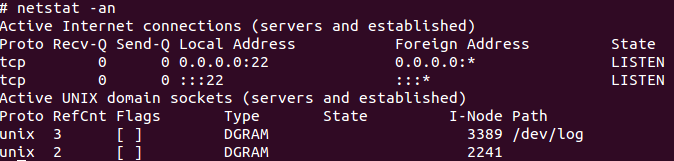
\includegraphics[width=14cm]{netstat_scapy.png}
\end{center}
\vspace{0.5cm}



\pagebreak
\subsection{Command "hping3"}
Comme le script Scapy ne fonctionnait pas très bien, nous avons décidé de tester un autre outil : "hping3". Les résultats sont très concluant. Voici la commande utilisée pour générer l'attaque :
\begin{lstlisting}[frame=single,style=Console]  % Start your code-block

hping3 --flood -I eth0 -V --rand-source -S -p 22 192.168.0.11
\end{lstlisting}

Cette commande générer des attaque de type TCP SYN, avec un port de source aléatoire et l'envoie le plus rapidement possible. Il faut être rapide, car la carte embarquée l'est aussi (8 coeurs!).

Voici la liste des ports ouverts sans la protection contre ce type d'attaques :
\begin{center} 
\hspace{15cm}
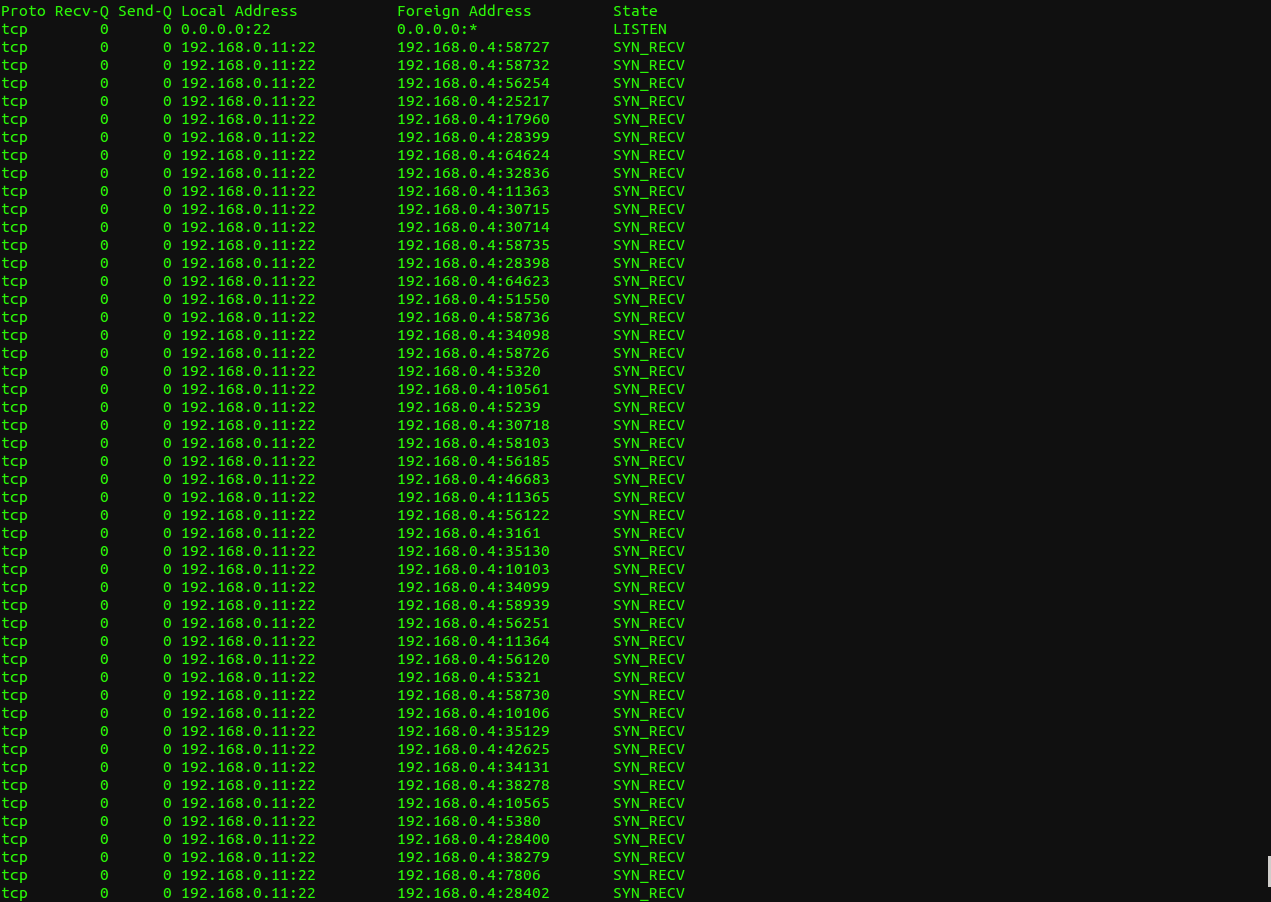
\includegraphics[width=16cm]{tcpsynCookie.png}
\end{center}
\vspace{0.5cm}

\pagebreak
Et si on active la protection : 
\begin{lstlisting}[frame=single,style=Console]  % Start your code-block

echo 1 > /proc/sys/net/ipv4/tcp_syncookies
\end{lstlisting}

Voilà le résultat :
\begin{center} 
\hspace{15cm}
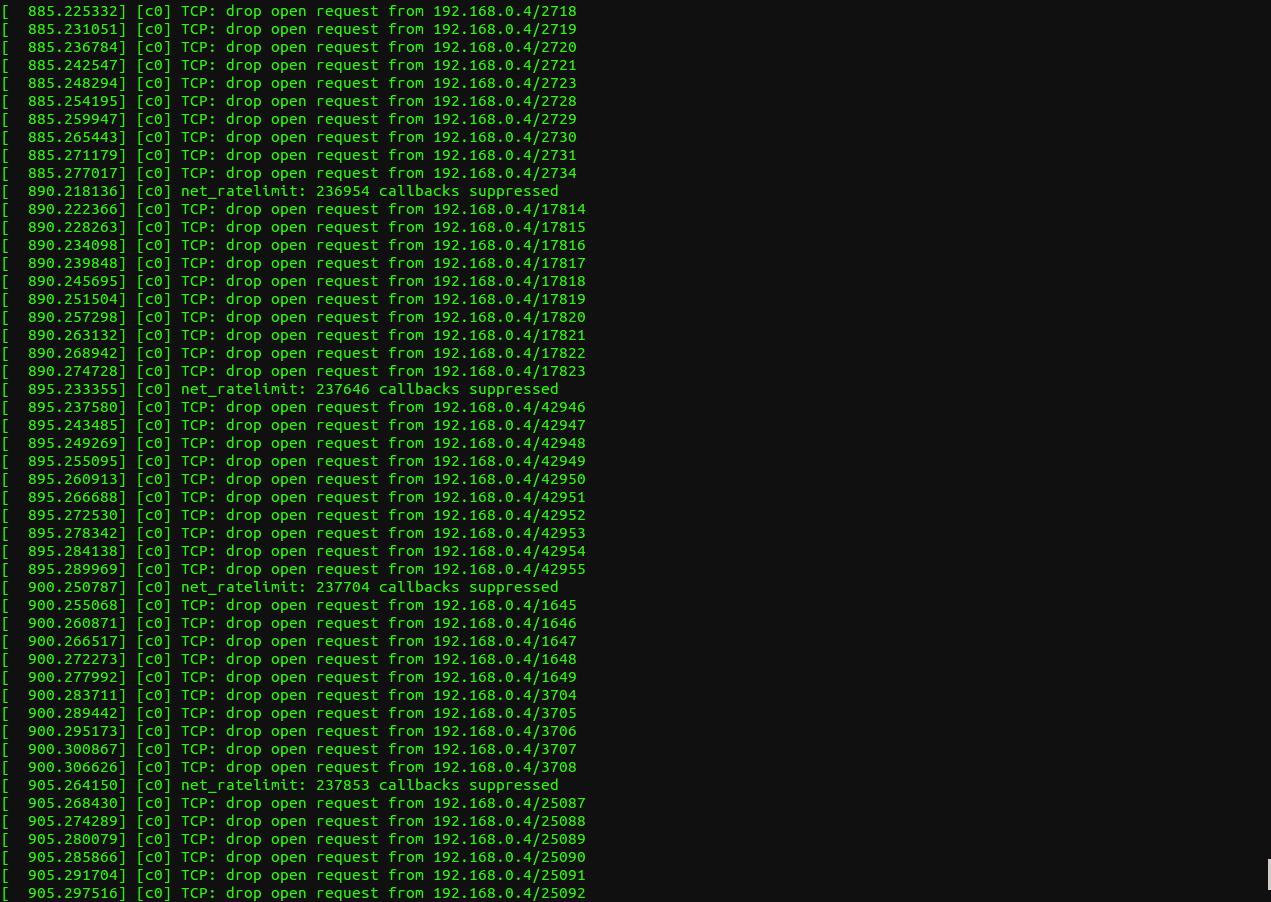
\includegraphics[width=16cm]{tcpSyn_protection.png}
\end{center}
\vspace{0.5cm}

On voit que le noyau rejette les connexions au fur et a mesure qu'elles arrivent et ne se terminent jamais.


